\documentclass{beamer}
\mode<presentation>
{
	\usetheme{Madrid}      % or try Darmstadt, Madrid, Warsaw, ...
	\usecolortheme{dolphin} % or try albatross, beaver, crane, ...
	\usefonttheme{serif}  % or try serif, structurebold, ...
	\setbeamertemplate{navigation symbols}{}
	\setbeamertemplate{caption}[numbered]
} 

\usepackage{graphicx} % Allows including images
\usepackage[utf8]{inputenc} % non-ASCII input
\usepackage[OT1]{fontenc}
\usepackage{relsize} % change long formula font size
\usepackage{amsmath,amssymb,amsthm,amsfonts,bm,bbm}
\usepackage{enumerate}
\usepackage[nodayofweek,level]{datetime}
\newdate{date}{13}{05}{2019}

\usepackage{natbib}

\DeclareMathOperator*{\argmin}{arg\,min}
\DeclareMathOperator*{\argmax}{arg\,max}

\newcommand{\EX}{\mathbb{E}} % expected value
\newcommand{\bnw}{\widehat{\bm{\beta}}_n^w} % weighted lasso estimator
\newcommand{\bhat}{\widehat{\bm{\beta}}_n} % strongly consistent estimator
\newcommand{\bLAS}{\widehat{\bm{\beta}}_n^{\text{LAS}}} % lasso estimator
\newcommand{\bLS}{\widehat{\bm{\beta}}_n^{\text{OLS}}} % LSE 
\newcommand{\be}{\bm{\beta}} % beta vector
\newcommand{\ep}{\bm{\epsilon}} % epsilon vector
\newcommand{\eLS}{\bm{e}_n^{\text{OLS}}} % LSE residual vector
\newcommand{\sumin}{\sum_{i=1}^n} % sum from i = 1 to n
\newcommand{\dn}{\frac{1}{n}} % 1/n
\newcommand{\dqn}{\frac{1}{\sqrt{n}}} % 1/sqrt{n}
\newcommand{\CONV}[1]{\stackrel{\text{#1}}{\longrightarrow}} % convergence mode
\newcommand{\overbar}[1]{\mkern 2mu\overline{\mkern-2mu#1\mkern-2mu}\mkern 2mu}
\newcommand{\x}{\bm{x}_i} % i-th row of design matrix X

\newcommand{\light}[1]{\textcolor{lightgray}{#1}}

%----------------------------------------------------------------------------------------
%	TITLE PAGE
%----------------------------------------------------------------------------------------

\title[Random-weighting]{Random-weighting in LASSO Regression} % The short title appears at the bottom of every slide, the full title is only on the title page

\subtitle{Institute for Foundations of Data Science (IFDS) Seminar}

\author{Tun Lee Ng \and Michael A. Newton} 

\date{\displaydate{date}} 

%----------------------------------------------------------------------------------------
%	Auto-generate content page at each section
%----------------------------------------------------------------------------------------


\AtBeginSection[]
{
	\begin{frame}<beamer>
	\frametitle{Outline}
	\tableofcontents[currentsection,currentsubsection]
	\end{frame}
\addtocounter{framenumber}{-1}% If you don't want them to affect the slide number
}

%----------------------------------------------------------------------------------------
%	Begin!
%----------------------------------------------------------------------------------------

\begin{document}

\begin{frame}
\titlepage
\end{frame}

\section{Motivation}

\begin{frame}{Motivation}
	\begin{itemize}
		\item data : $\bm{y} = (y_1, \ldots, y_n)$ 
		\item parameters : $\bm{\theta} = (\theta_1, \ldots, \theta_p)$ 
		\item Bayes : $p(\bm{\theta}|\bm{y}) \propto p(\bm{y}|\bm{\theta}) p(\bm{\theta})$
	\end{itemize}
	\vspace{0.3cm}
	MCMC:
	\begin{itemize}
		\item works well for moderate-sized models
		\item computationally intensive \& mixing hard to verify for large models 
	\end{itemize} 
	\vspace{0.3cm}
	Optimization:
	\begin{itemize}
		\item Efficient algorithms available 
		\item Optimization feasible in many models, eg. MAP estimation
		$$
		\widehat{\bm{\theta}} = \argmax_{\bm{\theta}} p(\bm{\theta}|\bm{y})
		$$ 
	\end{itemize}
	\vspace{0.3cm}
	Q: Any alternative method to obtain posterior samples?\\
	A: How about random-weighting \citep{WBB} \\
	\vspace{0.2cm}
\end{frame}

\begin{frame}{Motivation}
	Example 1: Diabetes Study \citep{BayesianLasso}
	\begin{figure}[h]
		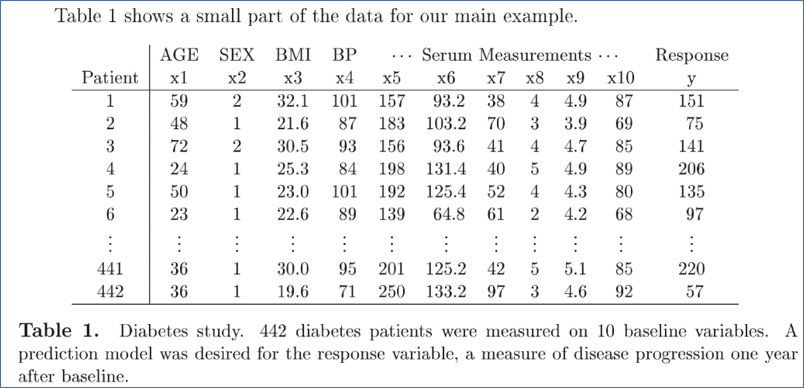
\includegraphics[scale=0.35]{Fig1}
	\end{figure}
	Random-weighting with LASSO regression \citep{WBB}: \\
	\vspace{0.3cm}
	\begin{small}
		For $j = 1, \ldots, B$,
		\begin{enumerate}
			\item Draw random weights $W_{j1},  \ldots, W_{jn} \stackrel{iid}{\sim} Exp(1)$.
			\item Solve $\widehat{\be}_{n(j)}^w = \argmin_{\be} \left\{ \sumin W_{ji} ( y_i - \x' \be )^2 + \lambda_n \sum_{j=1}^p |\beta_j| \right\}$.
		\end{enumerate}
	\end{small}
\end{frame}

\begin{frame}{Motivation}
	\begin{tiny}
		Example 1: Diabetes Study \citep{BayesianLasso}; Random-weighting \citep{WBB} 
	\end{tiny}
	\begin{figure}[h]
		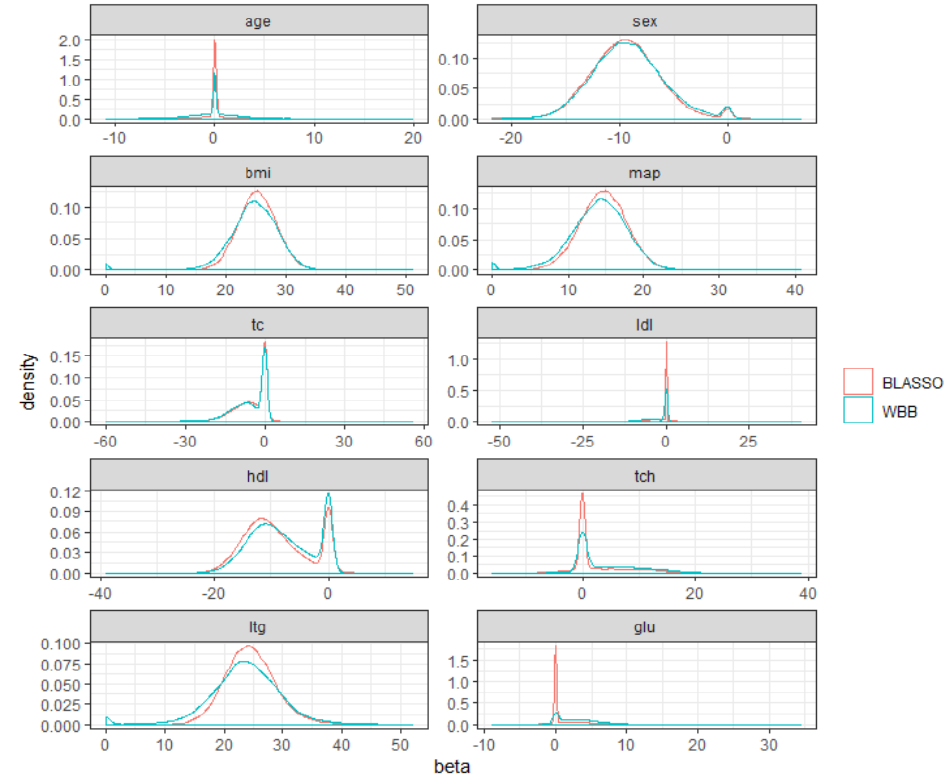
\includegraphics[scale=0.47]{Fig3}
	\end{figure}
\end{frame}

\section{Main Results}

\begin{frame}{Setup}
	$$
	Y = X \beta + \epsilon
	$$
	\begin{itemize}
		\item $\{\epsilon_i\}$ iid with mean 0, variance $\sigma^2_\epsilon$, and finite $4^{th}$ moment.
		\item All predictors are bounded.
		\item $\beta = (\beta_1, \ldots, \beta_p)'$ sparse.
		\item WLOG, partition $\be_0' = \left[\bm{\beta}'_{0(1)} \,\, \bm{\beta}'_{0(2)} \right]$, where 
		\begin{itemize}
			\item[--] $\bm{\beta}_{0(1)}$ is $q \times 1$ vector of true non-zero regression parameters,
			\item[--] $\bm{\beta}_{0(2)}$ is $(p-q) \times 1$ vector of zeroes.
		\end{itemize} 
		\item $q$ is fixed.
		\item Correspondingly, partition $X = [X_{(1)} \,\, X_{(2)}]$, and denote
		$$
		C_{n(11)} = \frac{1}{n} X'_{(1)} X_{(1)} 
		\qquad 
		\text{and} 
		\qquad
		C_{n(21)} = \frac{1}{n} X'_{(2)} X_{(1)} 
		$$
	\end{itemize}
\end{frame}

\begin{frame}{Main Results}
	$$
	\bnw = \argmin_{\be}
	\left\{
	\sumin W_i ( y_i - \x' \be )^2 
	+ \lambda_n \sum_{j=1}^p |\beta_j|
	\right\},
	\quad \text{where} \quad
	W_i \stackrel{iid}{\sim} Exp(1). 
	$$
	\vspace{1em}
	
	Conditional on data, $\bnw$ has the following properties: 
	\begin{itemize}
		\item conditional consistency (for fixed $p$) 
		\item conditional asymptotic normality (for fixed $p$) 
		\item conditional model selection consistency (for both fixed $p$ and growing $p_n$).
	\end{itemize}
\end{frame}

\begin{frame}{Main Results}
	\begin{block}{Theorem 1}
		$p$ is fixed. Assume $\frac{1}{n} X' X \to C$ for some non-singular $C$. 
		\begin{itemize}
			\item [ (a) ] \textbf{(Conditional Consistency)} If $\dfrac{\lambda_n}{n} \to 0$, then
			$$
			\bnw \CONV{c.p.} \bm{\beta}_0 \quad a.s. \,\, P_D.
			$$
			\item [ (b) ] 	If $\dfrac{\lambda_n}{n} \to \lambda_0 \in (0,\infty)$, then 
			$$
			\left( \bnw - \bm{\beta}_0 \right) \CONV{c.p.} \argmin_{\bm{u}} g(\bm{u}) \quad a.s. \,\, P_D,
			$$
			where
			\begin{align*} 
			g(\bm{u}) = \bm{u}' C \bm{u} 
			+ \lambda_0 \| \bm{\beta}_0 + \bm{u} \|_1 .
			\end{align*}  
		\end{itemize} 
	\end{block}
\end{frame}

\begin{frame}{Main Results}
	\begin{block}{Theorem 2 (Asymptotic Conditional Distribution)}
		$p$ is fixed. Assume $\frac{1}{n} X' X \to C$ for some non-singular $C$. If $\frac{\lambda_n}{\sqrt{n}} \to 0$, then
		$$
		\sqrt{n} \left( 
		\bnw - \bLS 
		\right) 
		\CONV{c.d.} 
		N \left( \bm{0}, \sigma^2_{\epsilon} C^{-1} \right)
		\quad a.s. \,\, P_D,
		$$
		where $\bLS$ is the ordinary least squares estimator of $\be$ in the linear model. 	 
	\end{block}
\end{frame}

\begin{frame}{Main Results}
	\begin{block}{Theorem 3 (Posterior Model Selection Consistency) -- fixed $p$}
		Assume $\frac{1}{n} X' X \to C$ for some non-singular $C$, and the \textbf{strong irrepresentable condition} \citep{BinYu}  
		\begin{align*} 
		\left|
		C_{n(21)} 
		\left( C_{n(11)} \right)^{-1} 
		\text{sgn} \left( \bm{\beta}_{0(1)} \right)
		\right| \leq
		\bm{1} - \bm{\eta},
		\end{align*}
		where inequality holds element-wise, and $0 < \eta_j \leq 1$ $\forall$ $j = 1, \cdots, p-q$. Then, for any $\frac{1}{2} < c_1,c_2 < 1$ such that $c_1 + c_2 < 1.5$, and for all $\lambda_n$ that satisfies 
		$$
		\dfrac{\lambda_n}{n^{c_2}} \to \infty
		\qquad \text{but} \qquad
		\dfrac{\lambda_n}{n^{1.5 - c_1}} \to 0,
		$$
		we have
		$$
		P\left(
		\bnw (\lambda_n) \stackrel{s}{=} \bm{\beta}_0
		\big| \mathcal{F}_n 
		\right)	
		\to 1
		\quad a.s. \,\, P_D.
		$$ 
	\end{block}
\end{frame}

\begin{frame}{Main Results}
	\begin{block}{Theorem 4 (Posterior Model Selection Consistency) -- growing $p_n$}
		Assume the \textbf{strong irrepresentable condition} \citep{BinYu}, and that for some $M_2 >0$, 
		$$
		\bm{\alpha}' 
		C_{n(11)}
		\bm{\alpha}
		\geq M_2
		\quad
		\forall
		\quad
		\Vert \bm{\alpha} \Vert_2 = 1.
		$$
		For any $0 < c_3 < \frac{1}{2} < c_1 , c_2 < 1$ such that $c_3 < 2 \min(c_1, c_2) -  1$ and $c_1 + c_2 < 1.5$, for which $p_n = \mathcal{O} \left( n^{c_3} \right)$ and $\lambda_n = \mathcal{O} \left( n^{c_2} \right)$, we have
		$$
		P\left(
		\bnw (\lambda_n) \stackrel{s}{=} \bm{\beta}_0
		\big| \mathcal{F}_n 
		\right)	
		\to 1
		\quad a.s. \,\, P_D. 
		$$  	
	\end{block}
\end{frame}

\begin{frame}{Connection to Bayesian Approach}
\begin{itemize}
	\item If $\lambda_n = o (\sqrt{n})$, first-order approximation to Bayesian samples.
	\item If $\lambda_n = \mathcal{O} (n^c)$ for $\frac{1}{2} < c < 1$, posterior model selection consistency.
\end{itemize}
\end{frame}

\section{Other Issues}

\subsection{Non-Standard-Exponential Weights}

\begin{frame}{Non-Standard-Exponential Weights}
Q: What if $W_i$ is any positive r.v. with $\mu_W = \sigma^2_W = 1$ and $\mathbb{E} (W_i^4) < \infty$? \\
A: Same asymptotic results in Theorems 1 - 3. \\
\vspace{1.2cm}
Q: What if $\mu_W$  and/or $\sigma^2_W$ not equal to 1? \\
A: Nice properties like Theorems 1 - 4, with asymptotics scaled accordingly with $\mu_W$  and $\sigma^2_W$. 
\end{frame}

\subsection{Weighting the Penalty Term} 

\begin{frame}{Weighting the Penalty Term}
Q: What if 
\begin{enumerate}
	\item $\bnw = 
		\argmin_{\be} 
		\left\{ 
			\sumin W_i ( y_i - \x' \be )^2 
			+ \lambda_n W_0 \sum_{j=1}^p |\beta_j| 
		\right\}$
	\item $\bnw = 
		\argmin_{\be} 
		\left\{ 
			\sumin W_i ( y_i - \x' \be )^2 
			+ \lambda_n \sum_{j=1}^p W_j |\beta_j| 
		\right\}
$\end{enumerate}
\vspace{0.5cm}
A: Nice properties like Theorems 1 - 4, with penalty terms in asymptotics weighted accordingly. 
\end{frame}

\section{Future Work}

\begin{frame}{Future Work}
\begin{itemize}
	\item Growing $p_n$?
	\item Other likelihood and/or penalty structure?
\end{itemize}
\end{frame}

\begin{frame}[noframenumbering]{References}
	\bibliographystyle{asa}	
	{\footnotesize
		\bibliography{IFDS_ref}        
	} 
\end{frame}

\end{document}